\documentclass{article}
\usepackage[left=4cm, right=4cm, top=4cm, bottom=4cm]{geometry}
\usepackage[T1]{fontenc}
\usepackage[polish]{babel}
\usepackage{graphicx}

\title{JIMP2 Projekt 2025 \\ {\large Dokumentacja funkcjonalna - C}}
\author{Michał Ludwiczak, Łukasz Leśniak \\ GR3}
\date{11 marca 2025}

\begin{document}

\maketitle

% Dokumentacja ma opisywać działanie projektu.



% proponowany cel projektu (nieprzepisany z opisu zadania przez prowadzącego),
\section{Cel projektu}

Celem projektu jest stworzenie aplikacji w języku C, dokonującej podziału grafu na określoną przez użytkownika lub domyślną liczbę 2 równych części z zachowaniem wybranego lub, ponownie, domyślnego 10-procentowego marginesu różnicy. Liczba wierzchołków w powstałych częściach grafu nie powinna się różnić o więcej niż zadany margines procentowy, a liczba przeciętych krawędzi pomiędzy wierzchołkami grafu powinna być jak najmniejsza. Wyjściem programu ma być plik tekstowy lub binarny. Użytkownik ma mieć możliwość wskazać wyjście programu, a więc plik tekstowy lub binarny, zawierający wynik działania programu, oraz dane wejściowe, które mogą być wykorzystane ponownie w kolejnym działaniu programu.



% wizualizacja problemu
\begin{figure}[ht]
    \centering
    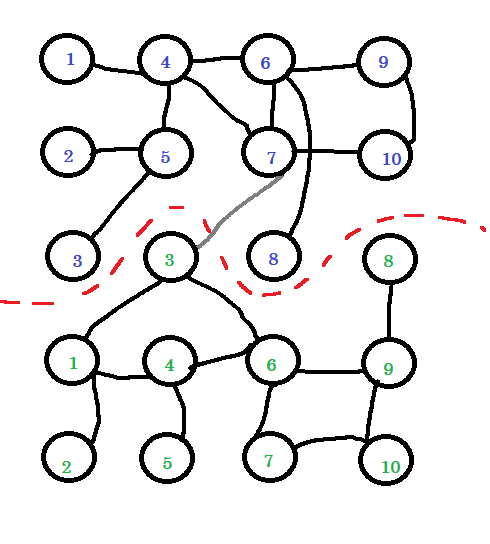
\includegraphics[width=0.5\linewidth]{graph.png}
    \caption{Przykładowy graf podzielony na 2 równe części\%}
    \label{fig:graph}
\end{figure}



% Opis funkcji udostępnianych przez program
\section{Funkcjonalności programu}

Program umożliwia użytkownikowi:

\begin{itemize}
    \item \textbf{Wczytanie grafu} z pliku tekstowego zgodnego z określonym formatem wejściowym.
    \item \textbf{Podział grafu} na zadaną liczbę części, minimalizując liczbę przeciętych krawędzi.
    \item \textbf{Określenie} dopuszczalnego \textbf{marginesu} procentowego różnicy w liczbie wierzchołków między częściami.
    \item \textbf{Zapisanie wyniku} działania programu w pliku tekstowym lub binarnym, umożliwiającym ponowne wykorzystanie danych wejściowych.
    \item \textbf{Obsługę błędów}, takich jak: niepoprawny format wejściowy, brak wymaganych argumentów czy brak pliku wejściowego.
\end{itemize}



% Lista dostępnych flag sterujących programem, wraz z dokładnym opisem dopuszczalnych wartości argumentów tych flag
\section{Flagi i argumenty}

Program jest uruchamiany z linii poleceń i obsługuje następujące flagi:

\begin{description}
    \item[<plik\_wejściowy>] \hfill \\
    \textbf{input} \\
    Ścieżka do pliku wejściowego zawierającego opis grafu. \\
    \textit{Wymagane jako pierwszy argument}
    
    \item[-p \texttt{<liczba\_części>}] \hfill \\
    \textbf{parts} \\
    Określa liczbę części, na które ma zostać podzielony graf. \\
    \textit{Domyślnie:} 2
    
    \item[-m \texttt{<margines>}] \hfill \\
    \textbf{margin} \\
    Określa dopuszczalny margines procentowy różnicy w liczbie wierzchołków między częściami. \\
    \textit{Domyślnie:} 10\%
    
    \item[-o \texttt{<plik\_wyjściowy>}] \hfill \\
    \textbf{output} \\
    Określa ścieżkę do pliku wyjściowego, w którym zostaną zapisane wyniki. \\
    \textit{Domyślnie:} output.txt
    
    \item[-f \texttt{<format\_pliku\_wyjściowego>}] \hfill \\
    \textbf{format} \\
    Określa format pliku wyjściowego: \texttt{txt} dla pliku tekstowego lub \texttt{bin} dla pliku binarnego. \\
    \textit{Domyślnie:} txt
\end{description}



% jeżeli program akceptuje niestandardowe formaty danych należy je opisać
\section{Format danych wejściowych}

Program akceptuje pliki wejściowe z rozszerzeniem .csrrg. Format danych wejściowych jest zdefiniowany za pomocą 5 linijek, z których każda odpowiada za zapis informacji. \\

\begin{enumerate}
    \item Maksymalna możliwa liczba węzłów w wierszu (w grafie mogą być wiersze o ich mniejszej liczbie, ale nie o większej).
    \item Indeksy węzłów w poszczególnych wierszach – liczba wszystkich indeksów odpowiada liczbie węzłów grafu.
    \item Wskaźniki na pierwsze indeksy węzłów w liście wierszy z poprzedniego punktu.
    \item Grupy węzłów połączone przy pomocy krawędzi.
    \item Wskaźniki na pierwsze węzły w poszczególnych grupach z poprzedniego punktu. Ta sekcja może występować w pliku wielokrotnie, co oznacza, że plik zawiera więcej niż jeden graf.
\end{enumerate}




\section{Przykłady wywołania programu}

Poniżej przedstawiono przykłady wywołania programu wraz z opisem konfiguracji poszczególnych parametrów.

\begin{itemize}
    \item \texttt{./program graf.csrrg} \\
    Wczytuje plik wejściowy \texttt{graf.csrrg} i dzieli graf na 2 części (domyślnie), z marginesem 10\% i zapisuje wynik do \texttt{output.txt} w formacie tekstowym.
    
    \item \texttt{./program graf.csrrg -p 3 -m 5} \\
    Wczytuje plik wejściowy \texttt{graf.csrrg} i dzieli graf na 3 części, dopuszczając maksymalnie 5\% różnicy w liczbie wierzchołków między częściami. Wynik zostanie zapisany do \texttt{output.txt} w formacie tekstowym.
    
    \item \texttt{./program graph.csrrg -o wynik.bin -f bin} \\
    Wczytuje plik wejściowy \texttt{graph.csrrg}, dzieli graf na 2 części (domyślnie), z marginesem 10\% i zapisuje wynik do pliku binarnego \texttt{wynik.bin}.
    
    \item \texttt{./program graf3.csrrg -p 4 -m 15 -o podzial.txt -f txt} \\
    Wczytuje plik wejściowy \texttt{graf3.csrrg} i dzieli graf na 4 części, dopuszczając maksymalnie 15\% różnicy w liczbie wierzchołków między częściami. Wynik zostanie zapisany do \texttt{podzial.txt} w formacie tekstowym.
\end{itemize}



% przegląd sytuacji wyjątkowych obsługiwanych przez program (komunikaty z wytłumaczeniem sytuacji oraz ew. kod powrotu programu)
\section{Obsługa sytuacji wyjątkowych}

Program ma być zaprojektowany tak, aby w przypadku wystąpienia błędów informować użytkownika za pomocą czytelnych komunikatów. Poniżej przedstawiono listę możliwych błędów, ich opis oraz sugerowane działania:

\begin{itemize}
    \item \textbf{Brak ścieżki do pliku wejściowego} \\
    \textbf{Komunikat:} Błąd: Nie podano ścieżki do pliku wejściowego jako argument. \\
    \textbf{Opis:} Program został uruchomiony bez podania ścieżki do pliku wejściowego jako pierwszy argument, która jest niezbędna.

    \item \textbf{Niepoprawny format pliku wejściowego} \\
    \textbf{Komunikat:} Błąd: Niepoprawny format pliku wejściowego. \\
    \textbf{Opis:} Plik wejściowy nie spełnia oczekiwanego formatu. Sprawdź, czy plik jest zgodny z określonym formatem danych wejściowych.

    \item \textbf{Brak pliku wejściowego} \\
    \textbf{Komunikat:} Błąd: Nie znaleziono pliku wejściowego. \\
    \textbf{Opis:} Określony plik wejściowy nie istnieje w podanej lokalizacji. Zweryfikuj ścieżkę do pliku lub upewnij się, że plik został utworzony.

    \item \textbf{Niepoprawna wartość liczby części} \\
    \textbf{Komunikat:} Błąd: Liczba części musi być większa niż 1. \\
    \textbf{Opis:} Podana liczba części do podziału grafu jest mniejsza lub równa 1. Wprowadź wartość większą niż 1.

    \item \textbf{Niepoprawna wartość marginesu} \\
    \textbf{Komunikat:} Błąd: Margines musi być liczbą z zakresu 0-100. \\
    \textbf{Opis:} Wartość marginesu znajduje się poza dozwolonym zakresem. Upewnij się, że margines jest liczbą całkowitą między 0 a 100.

    \item \textbf{Błąd zapisu pliku wyjściowego} \\
    \textbf{Komunikat:} Błąd: Nie można zapisać do pliku wyjściowego. \\
    \textbf{Opis:} Program napotkał problem podczas próby zapisania wyników do pliku wyjściowego. Sprawdź uprawnienia do zapisu w docelowej lokalizacji lub wybierz inną ścieżkę.

    \item \textbf{Błąd podczas podziału grafu} \\
    \textbf{Komunikat:} Błąd: Nie udało się podzielić grafu. \\
    \textbf{Opis:} Program napotkał problem podczas próby podziału grafu.
\end{itemize}



\end{document}
